\documentclass[12pt]{article}
\usepackage[english]{babel}
\usepackage{subcaption}
\usepackage{hyperref}
\usepackage{graphicx}
\graphicspath{{images/}}
\usepackage{geometry}
 \geometry{
 a4paper,
 total={170mm,257mm},
 left=20mm,
 top=20mm,
 }
\begin{document}

\section{Problem1}
In the first problem, we are supposed to enhance the quality of the given input video.

\subsection{Method Employed}
\begin{enumerate}
\item First we converted the image into gray and analyzed the pixel distribution using histogram and got the following output.

\begin{figure}[h]
    \centering
    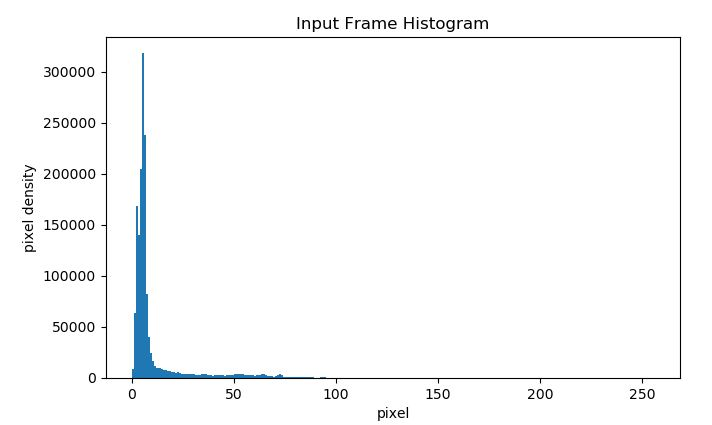
\includegraphics[width=12cm]{inputhistogramoutput}
    \caption{Input frame Histogram output}
    \label{fig:inputhistogramoutput}
\end{figure}

We saw high density of pixels within the range 0-50. The goal was to increase the contrast by distributing the pixel density evenly between 0-255.

\item Initially we tried to improve the quality of the video using histogram equalization. The output certainly increased the brightness of the video but at the same time amplified also noise.

\begin{figure}[h]
    \centering
    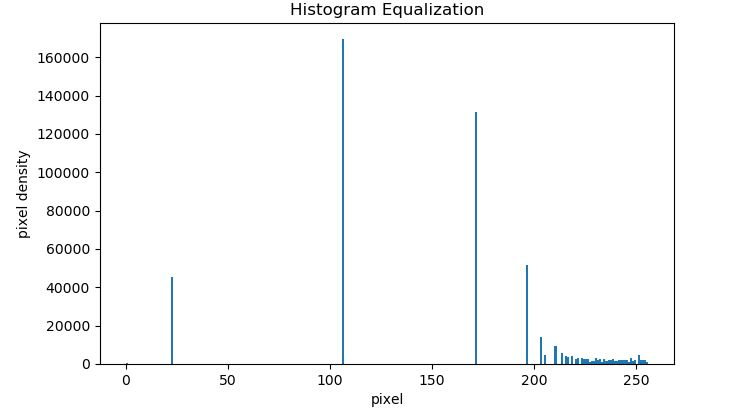
\includegraphics[width=12cm]{histogramequalization}
    \caption{Histogram Equalization output}
    \label{fig:histogramequalization}
\end{figure}

After performing histogram equalization, the pixel density was distributed but resulted in noise amplification clearly seen between pixel range 100-150. We tried to decrease the noise by using filters but could not decrease the noise.

\item We employed gamma correction. This method could increase the quality by could not increase the contrast.
\begin{figure}[h]
    \centering
    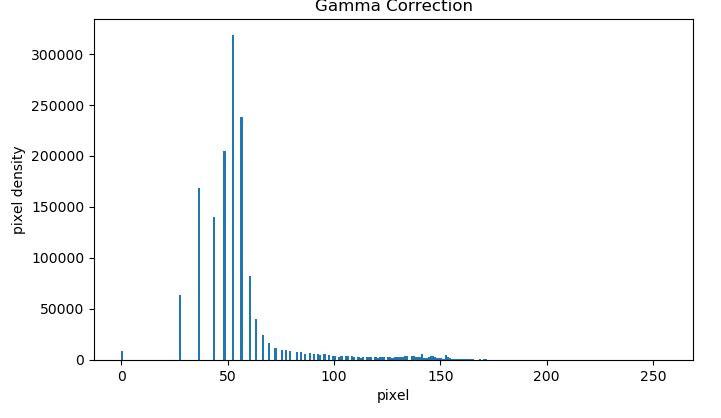
\includegraphics[width=12cm]{gammahist}
    \caption{Gamma Correction output}
    \label{fig:gammahist}
\end{figure}

\item Then we multiplied each pixel with $\alpha$ and added by $\beta$. We found this method increased the contrast while decreasing the noise compared to histogram equalization. The histogram output of this method is given below:

\begin{figure}[h]
    \centering
    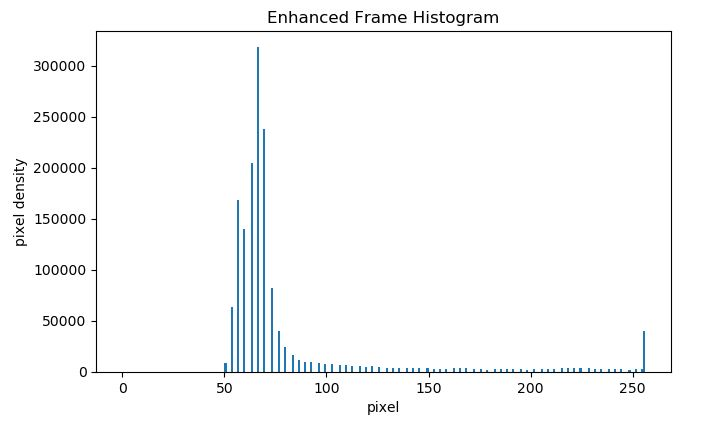
\includegraphics[width=12cm]{enhancedhistogram}
    \caption{Enhanced Frame output}
    \label{fig:enhancedhistogram}
\end{figure}
We can see that the pixel density is distributed and at 255 there is sharp rise in the pixel density which is indicative of increase in contrast of the image. The equation below clearly outlines this method:
\begin{equation}
	NewFrame = \alpha*OldImage + \beta
\end{equation}
\end{enumerate}

\subsection{Outputs Obtained}
\begin{enumerate}
\item The outputs are snippets of one of the input frame taken from the video. The input frame considered: 
\begin{figure}[h]
    \centering
    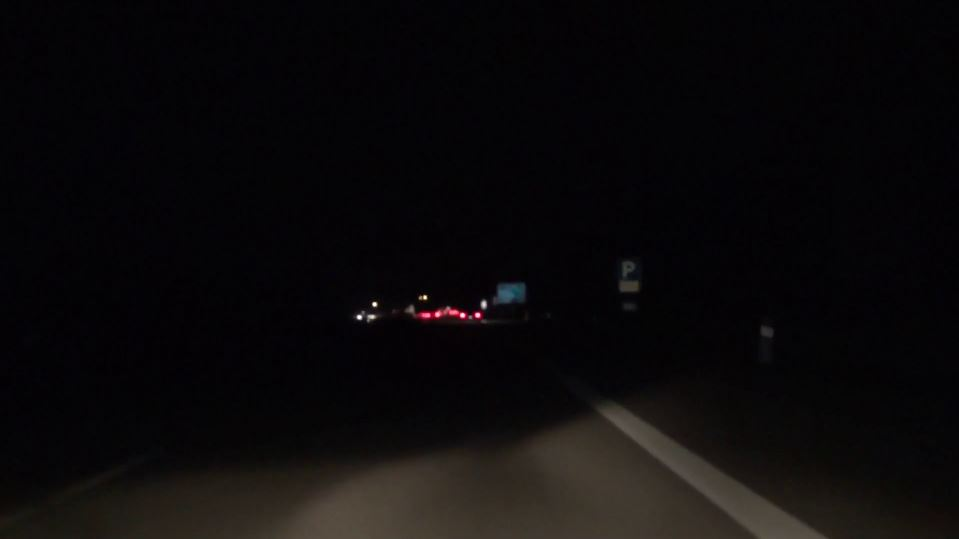
\includegraphics[width=14cm]{inputframe}
    \caption{Input Frame}
    \label{fig:inputframe}
\end{figure}

\item Histogram Equalization Output: This contains the snippet output obtained by employing histogram equalization. We can see that the contrast is improved at the same time noise is also improved.
\begin{figure}[h]
    \centering
    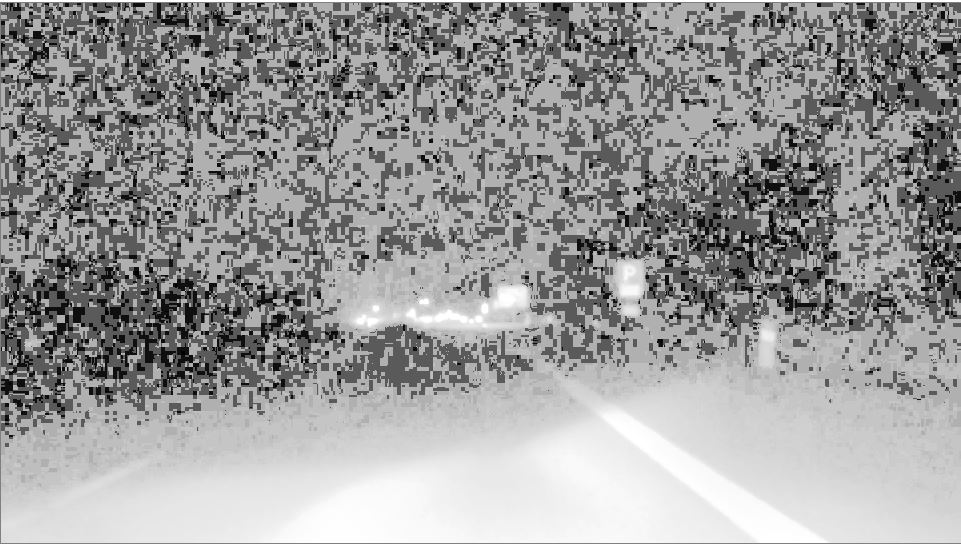
\includegraphics[width=14cm]{histequvideo}
    \caption{Histogram Equalization output}
    \label{fig:histequvideo}
\end{figure}

\newpage
\item Gamma Correction Output: This contains the snippet output obtained by employing Gamma correction. We can see that contrast is not improved.

\begin{figure}[h]
    \centering
    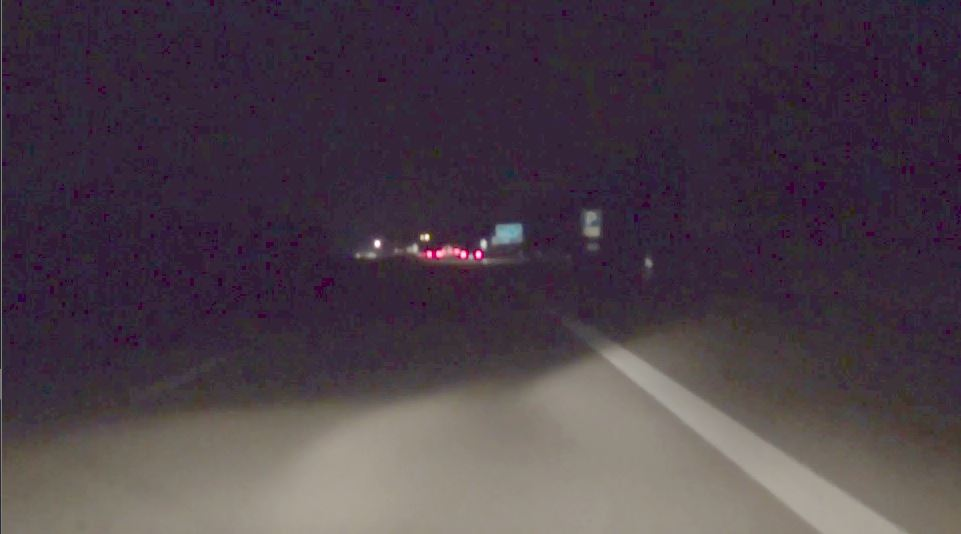
\includegraphics[width=14cm]{gammavideo}
    \caption{Gamma Correction output}
    \label{fig:gammavideo}
\end{figure}

\item Method Employed Output: This is the snippet of the image frame from the enhanced video. We improved the contrast and decreased the noise levels.We can clearly see the lanes and road signs from the enhanced frame.
\begin{figure}[h]
    \centering
    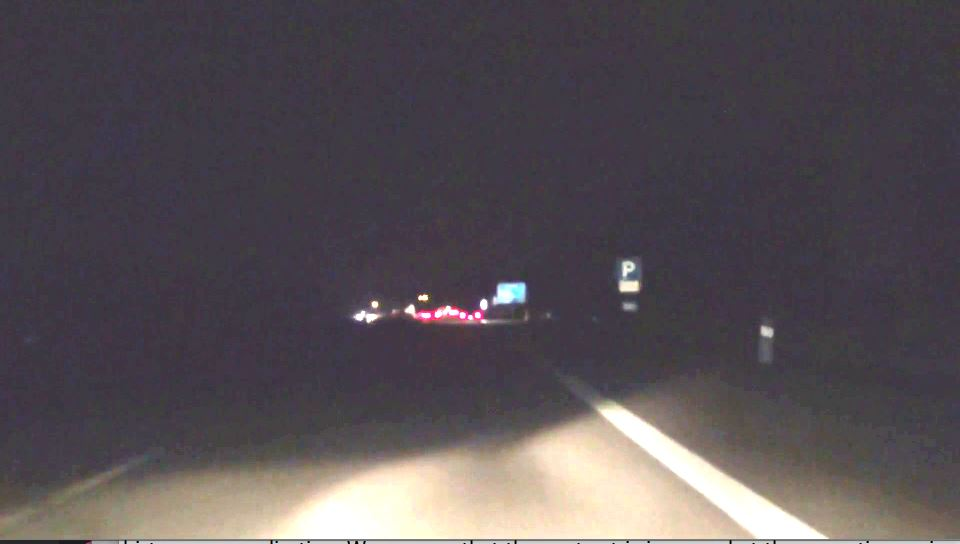
\includegraphics[width=14cm]{enhancedvideosnippet}
    \caption{Enhanced frame output}
    \label{fig:enhancedvideosnippet}
\end{figure}
\end{enumerate}

\subsection{Accessing output video} 
For accessing the full length output video please click on this \href{https://drive.google.com/drive/folders/1f6jBcJo96DZhwxBkdezf6MwAXwktGqS-?usp=sharing}{\underline{link}}.

\subsection{References:}
\begin{enumerate}
\item \href{https://docs.opencv.org/3.4/d3/dc1/tutorial_basic_linear_transform.html}{\underline{Opencv documentation for improving the contrast and quality of the image.}}

\end{enumerate}
\end{document}

